\documentclass{beamer}\usepackage{graphicx, color}
%% maxwidth is the original width if it is less than linewidth
%% otherwise use linewidth (to make sure the graphics do not exceed the margin)
\makeatletter
\def\maxwidth{ %
  \ifdim\Gin@nat@width>\linewidth
    \linewidth
  \else
    \Gin@nat@width
  \fi
}
\makeatother

\IfFileExists{upquote.sty}{\usepackage{upquote}}{}
\definecolor{fgcolor}{rgb}{0.2, 0.2, 0.2}
\newcommand{\hlnumber}[1]{\textcolor[rgb]{0,0,0}{#1}}%
\newcommand{\hlfunctioncall}[1]{\textcolor[rgb]{0.501960784313725,0,0.329411764705882}{\textbf{#1}}}%
\newcommand{\hlstring}[1]{\textcolor[rgb]{0.6,0.6,1}{#1}}%
\newcommand{\hlkeyword}[1]{\textcolor[rgb]{0,0,0}{\textbf{#1}}}%
\newcommand{\hlargument}[1]{\textcolor[rgb]{0.690196078431373,0.250980392156863,0.0196078431372549}{#1}}%
\newcommand{\hlcomment}[1]{\textcolor[rgb]{0.180392156862745,0.6,0.341176470588235}{#1}}%
\newcommand{\hlroxygencomment}[1]{\textcolor[rgb]{0.43921568627451,0.47843137254902,0.701960784313725}{#1}}%
\newcommand{\hlformalargs}[1]{\textcolor[rgb]{0.690196078431373,0.250980392156863,0.0196078431372549}{#1}}%
\newcommand{\hleqformalargs}[1]{\textcolor[rgb]{0.690196078431373,0.250980392156863,0.0196078431372549}{#1}}%
\newcommand{\hlassignement}[1]{\textcolor[rgb]{0,0,0}{\textbf{#1}}}%
\newcommand{\hlpackage}[1]{\textcolor[rgb]{0.588235294117647,0.709803921568627,0.145098039215686}{#1}}%
\newcommand{\hlslot}[1]{\textit{#1}}%
\newcommand{\hlsymbol}[1]{\textcolor[rgb]{0,0,0}{#1}}%
\newcommand{\hlprompt}[1]{\textcolor[rgb]{0.2,0.2,0.2}{#1}}%

\usepackage{framed}
\makeatletter
\newenvironment{kframe}{%
 \def\at@end@of@kframe{}%
 \ifinner\ifhmode%
  \def\at@end@of@kframe{\end{minipage}}%
  \begin{minipage}{\columnwidth}%
 \fi\fi%
 \def\FrameCommand##1{\hskip\@totalleftmargin \hskip-\fboxsep
 \colorbox{shadecolor}{##1}\hskip-\fboxsep
     % There is no \\@totalrightmargin, so:
     \hskip-\linewidth \hskip-\@totalleftmargin \hskip\columnwidth}%
 \MakeFramed {\advance\hsize-\width
   \@totalleftmargin\z@ \linewidth\hsize
   \@setminipage}}%
 {\par\unskip\endMakeFramed%
 \at@end@of@kframe}
\makeatother

\definecolor{shadecolor}{rgb}{.97, .97, .97}
\definecolor{messagecolor}{rgb}{0, 0, 0}
\definecolor{warningcolor}{rgb}{1, 0, 1}
\definecolor{errorcolor}{rgb}{1, 0, 0}
\newenvironment{knitrout}{}{} % an empty environment to be redefined in TeX

\usepackage{alltt}
\usetheme{Stats}
\setbeamercovered{transparent}
\usepackage{color}
\usepackage{hyperref}
  \hypersetup{
  	colorlinks=true
		linkcolor=black
		}
\usepackage{url}
\usepackage{graphics}
\usepackage{tikz}
\usepackage{booktabs}





%%%%%%%%%%%%%%%%%%%%%%%%%%%%%%%% Title Slide %%%%%%%%%%%%%%%%%%%%%%%%%%
\title[]{Intro to Social Science Data Analysis \\[1cm] Lecture 3:  Gathering Data}
\author[]{
    \href{mailto:gandrud@yonsei.ac.kr}{Christopher Gandrud}
}
\date{\today}


\begin{document}

\frame{\titlepage}

\section[Outline]{}
\frame{\tableofcontents}

\section{Recap}
\frame{
	\frametitle{Review}
  Last week we:
  \begin{itemize}
    \item Discussed why we care about data.
    \item Variables, observations, levels of measurement.
    \item Compared matrices to data frames.
    \item Learned basic data frame manipulation techniques.
  \end{itemize}
}

\begin{frame}[fragile]
  \frametitle{Quick Quiz 1}
  What {\bf{level of measurement}} are these variables at:
  \begin{enumerate}
    \item The number of people living in poverty in a city.
    \item Whether or not a country is at war.
    \item The names of a continent's major rivers.
  \end{enumerate}
\end{frame}

\begin{frame}[fragile]
  \frametitle{Quick Quiz 2}
  Comment this code:
\begin{knitrout}
\definecolor{shadecolor}{rgb}{0.969, 0.969, 0.969}\color{fgcolor}\begin{kframe}
\begin{alltt}
Subject <- \hlfunctioncall{c}(\hlstring{"A"}, \hlstring{"B"}, \hlstring{"C"})
Height <- \hlfunctioncall{c}(3.2, 4.5, 3.1)

Data <- \hlfunctioncall{data.frame}(Subject, Height)

DataB <- Data[2, ]
\end{alltt}
\end{kframe}
\end{knitrout}

\end{frame}


\section{Reminder: First Assignment}
\frame{
  \frametitle{First Assignment}
  {\large{{\bf{Due:}} Monday 24 September}} \\[0.5cm]
  Create a new data frame with country-level data from at least {\bf{two}} different sources. \\[0.5cm]
  Create a folder in your Dropbox and {\bf{email me the link}}. \\[0.5cm]
  The folder needs to include:
  \begin{enumerate}
    \item<1-> The new data frame saved as a \texttt{.csv} file.
    \item<1-> A text file {\bf{describing the variables and their sources}}.
    \item<1-> A notebook \texttt{.html} file detailing how you created the data frame and saved it as a\texttt{.csv}.
  \end{enumerate}
}

\frame{
  \frametitle{Marking Criteria}
  The assigment will be marked based on two criteria:
  \begin{enumerate}
    \item How well you gathered and merged the data so that the new data set can be used for {\emph{statistical analysis with minimal data loss}}.
    \item How well you {\emph{describe the data}} and {\emph{document your data gathering process}}. I should be able to understand your data, code, and all steps you took.
  \end{enumerate}
}

\frame{
  \frametitle{Using Dropbox}
  
}

\frame{
  \frametitle{This Week}
  {\LARGE{Last week we learned basic data frame handling skills. \\[0.5cm]
  But how do we usually {\bf{get data into R}} and make it {\bf{useable}} for data analysis?}}
}

\section{Data Gathering Principles}
\frame{
  \frametitle{Data Gathering Principles 1}
  {\LARGE{Populations}} \\[0.5cm]
  Your {\bf{research question}} should usually {\bf{guide your data gathering}}. \\[0.5cm]
  Your research question can indicate what the relevant {\bf{population}} is.
  \begin{itemize}
    \item<2-> Does income-level explain voting behaviour in Korea?
    \item<3-> Why do Southern European countries have higher deficits than Northern European ones?
    \item<4-> Why do civil wars happen?
  \end{itemize}
}

\frame{
  \frametitle{Data Gathering Principles 2}
  {\LARGE{Samples}} \\[0.5cm]
  It may {\bf{not be possible}} to gather data on the entire population of interest. \\[0.5cm]
  So we gather data on a subset of the population--a {\bf{sample}}.
}

\frame{
  \frametitle{Data Gathering Principles 3}
  {\LARGE{Anecdotal Evidence}} \\[0.5cm]
  If we want to answer questions about populations we should generally {\bf{avoid anecdotal evidence}}. For example: 
  \begin{itemize}
    \item<1-> The rich people I know vote for Party A not Party B.
  \end{itemize} \\[0.5cm]
  Anecdotal evidence is gathered in a {\bf{haphazard way}}. It is {\bf{not representative}} of the population and usually includes {\bf{extreme cases}}. \\[0.5cm]
  Because anecdotal evidence is not representative of the population of interest and {\bf{should not}} be used to make {\bf{generalizable}} conclusions.
}

\frame{
  \frametitle{Data Gathering Principles 3}
  {\LARGE{Random Sample}} \\[0.5cm]
  To avoid selecting extreme cases \& biasing our sample in other ways we should try to use {\bf{random sampling}}. \\[0.5cm]
  A sample is random if every member of a population has an {\bf{equal probability}} of being selected.
}

\frame{
  \frametitle{This Course}
  {\LARGE{Sampling in this Course}} \\[0.25cm]
  In this course we will mostly be using {\bf{observational data}}. \\[0.25cm]
  We will also usually use {\bf{convenience samples}} where we try to gather data on as much of the population as possible (attempt {\bf{exhaustability}}). \\[0.5cm]
  For example, if we want to research how democracy may affect economic development, we would try to gather data on
    \begin{itemize}
      \item<1-> level of democracy
      \item<1-> level of development
    \end{itemize}
  for {\bf{as many}} countries and years as we can.
}

\frame{
  \frametitle{Observational Data 1}
  {\LARGE{Sampling in this Course}} \\[0.25cm]
  Especially when we use convenience samples we {\bf{must always look out for factors that might bias our results}}. \\[0.5cm]
  We must be he honest. {\bf{Clearly state any potential biases in our presentation of results.}} \\[0.5cm]
  For example: \\[0.25cm]
  We wanted to study all countries, but usually found data only for wealthy countries.\\
  We need to clearly state that our findings might only be generalizable to wealthy countries, not all countries.
}

\frame{
  \frametitle{Observational Data 2}
  When we use observational data it is especially important to gather data not only on {\bf{what we want to explain}} and {\bf{what we think explains it}}, but also {\bf{other factors}} that may affect any relationship between these things that we might observe.
}

\section{Response \& Explanatory Variables}
\frame{
  \frametitle{Response Variables}
  The phenomenon we are interested in explaining is operationalized by the {\bf{response variable}}. \\[0.5cm]
  The response variable is also sometimes called the {\bf{dependent variable}} and denoted by $Y$.
  
}

\frame{
  \frametitle{Explanatory Variables}
  The factor we believe may explain our phenomenon of interest is operationalized by the {\bf{explanatory variable}}. \\[0.5cm]
  The explanatory variable is also sometimes called the {\bf{independent variable}} and denoted by $X$.
  
}

\frame{
  \frametitle{Response \& Explanatory Variables}
  \begin{figure}
    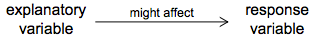
\includegraphics[scale = 0.6]{ExplainResponse.png}
    \begin{center}
      {\small{Source: Diaz et al. (2011, 29)}}
    \end{center}
  \end{figure}
}

\frame{
  \frametitle{Control Variables}
  However, {\bf{correlation does not equal causation}}. \\[0.5cm]
  In particular, we need to look out for {\bf{confounding factors}}. \\[0.25cm]
  Confounding factors are {\bf{associated with both}} the response and explanatory variables.
  \frametitle{Response \& Explanatory Variables}
  \begin{figure}
    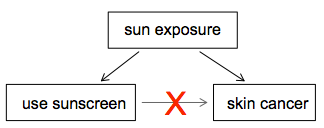
\includegraphics[scale = 0.6]{Confounder.png}
    \begin{center}
      {\small{Source: Diaz et al. (2011, 31)}}
    \end{center}
  \end{figure}
}

\frame{
  \frametitle{Control Variables \& Data Gathering 1}
  In parts II \& III of the course we look at ways to ``{\bf{control}}" for confounding factors. \\[0.5cm]
  At this point, when we gather data we need to consider not just the main response and explanatory variables, but also confounding factors. \\[0.5cm]
}
  
\frame{
  \frametitle{Control Variables \& Data Gathering 2}
  {\bf{Note:}} We want to control for as many confounders as possible, but there is a data gathering {\bf{trade off}}: \\[0.25cm]
  The more variables we gather, the more likely it is that we will have {\bf{missing data}}. \\[0.25cm]
  If data is {\bf{not missing at random}}, we will add sampling bias.
}

\section{Importing Data Into R}
\frame{
  \begin{center}
    {\LARGE{Ok, let's get some data into R.}}
  \end{center}
}

\frame{
  {\LARGE{Practical Tips}}
  \begin{itemize}
    \item Save your data as simple columns and rows (no fancy colours, etc.).
    \item Save it in a text format.
    \item Document:
      \begin{itemize}
        \item Where the data is from,
        \item What the variables mean,
        \item How you have changed it.
      \end{itemize}
  \end{itemize}
}

\frame{
  \frametitle{Simple Data Set}
  Data sets should be {\bf{simple}}. \\[0.25cm]
  If you open the data in Microsoft Excel:
    \begin{itemize}
      \item<2-> The {\bf{first row}} should have the variables names 
      \item<3-> The variable names should be simple and use the same rules as R object names.
      \item<4-> There should be no extra information or styling.
      \item<5-> If you have missing data cells should be empty or have NA.
    \end{itemize}
}

\frame{
  \frametitle{A Good Data Set}
  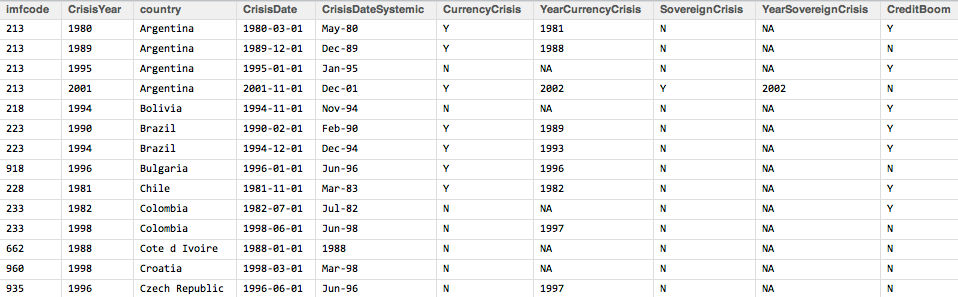
\includegraphics[scale = 0.5]{IdealData.png}
}

\frame{
  \frametitle{A Bad Data Set}
  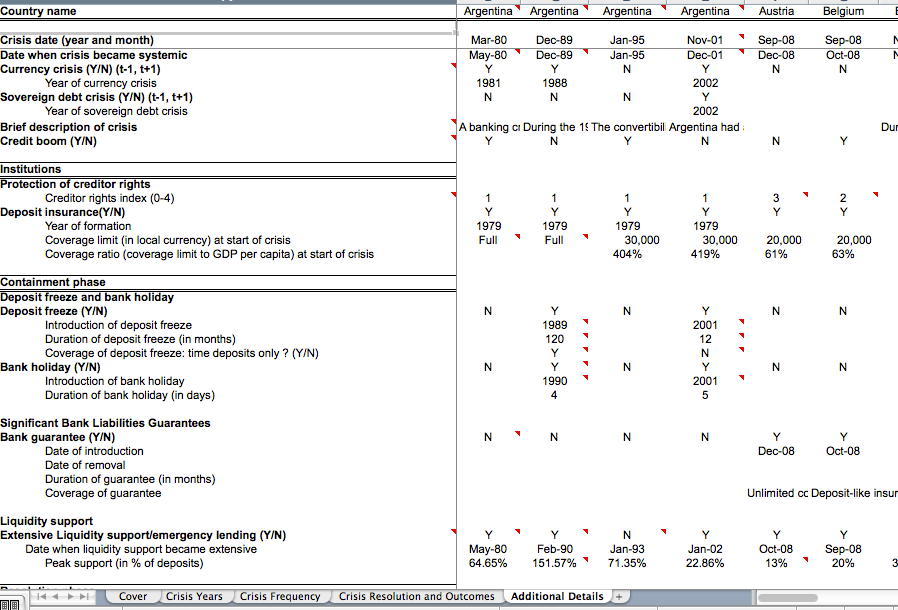
\includegraphics[scale = 0.5]{BadData.png}
}

\frame{
  \frametitle{Data in Text Files}
  You should save your data in a {\bf{plain text file format}}. \\[0.5cm]
  Plain-text file formats:
  \begin{itemize}
    \item<1-> Are simple,
    \item<1-> Can easily be loaded into R.
  \end{itemize} \\[0.5cm]
  My favourite is {\bf{comma seperated values (.csv)}}. 
}

\frame{
  \frametitle{Raw Plain-Text Data File}
  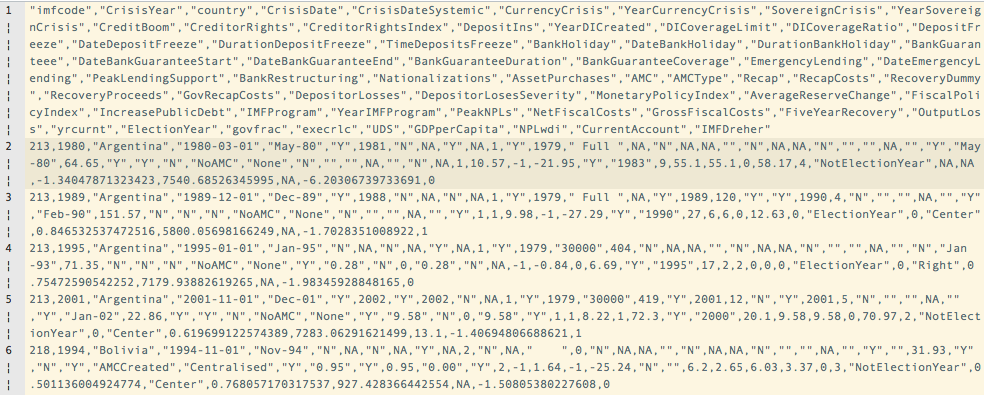
\includegraphics[scale = 0.5]{TextComma.png}
}

\frame{
  \begin{center}
    {\LARGE{Import Plain-Text Data}}
  \end{center}
}

\begin{frame}[fragile]
  \frametitle{Importing Plain-Text Data 1}
  Use the \texttt{read.table} command. \\[0.5cm]
  For example, if you have a file on your Desktop called MyFile.csv, load it like this:
\begin{knitrout}
\definecolor{shadecolor}{rgb}{0.969, 0.969, 0.969}\color{fgcolor}\begin{kframe}
\begin{alltt}
\hlcomment{# Import plain-text data into R}
NewData <- \hlfunctioncall{read.table}(file = \hlstring{"~/Desktop/Myfile.csv"}, 
    sep = \hlstring{","})
\end{alltt}
\end{kframe}
\end{knitrout}

\end{frame}

\begin{frame}[fragile]
  \frametitle{Importing Plain-Text Data 2}
\begin{knitrout}
\definecolor{shadecolor}{rgb}{0.969, 0.969, 0.969}\color{fgcolor}\begin{kframe}
\begin{alltt}
\hlcomment{# Import plain-text data into R}
NewData <- \hlfunctioncall{read.table}(file = \hlstring{"~/Desktop/Myfile.csv"}, 
    sep = \hlstring{","})
\end{alltt}
\end{kframe}
\end{knitrout}


  {\bf{Note:}}
  \begin{itemize}
    \item<1-> \texttt{"\textasciitilde{}/Desktop/Myfile.csv"} is the {\bf{directory}} $+$ {\bf{file name}}. This will be different depending on what operating system you have and where the file is.
    \item<2-> \texttt{sep = ","} tells R that the values in a row are seperated by commas
  \end{itemize}
\end{frame}

\frame{
  \begin{center}
    {\LARGE{Data from Other Statistics Programs}}
  \end{center}
}

\begin{frame}[fragile]
  \frametitle{Foreign Package}
  If you are importing data from another statistics program, such as SPSS or Stata, \texttt{foreign} packages. \\[0.5cm]
  For example, to load a Stata file with the {\bf{file extension}} \texttt{.dta}:
\begin{knitrout}
\definecolor{shadecolor}{rgb}{0.969, 0.969, 0.969}\color{fgcolor}\begin{kframe}
\begin{alltt}
\hlcomment{# Load foreign package library}
\hlfunctioncall{library}(foreign)
\hlcomment{# Load Stata data file MyFile.dta}
NewData <- \hlfunctioncall{read.dta}(file = \hlstring{"~/Desktop/Myfile.dta"})
\end{alltt}
\end{kframe}
\end{knitrout}

\end{frame}

\frame{
  \begin{center}
    {\LARGE{Data from Microsoft Excel}}
  \end{center}
}

\frame{
  \frametitle{Data from Excel, Practical Tips}
  If your data is in Excel format (i.e. \texttt{.xls})
  \begin{itemize}
    \item In Excel, simplify the data set (columns and rows, take out styling),
    \item Save it as a text file.
    \item Load using \texttt{read.table}
  \end{itemize}
}

\frame{
  \begin{center}
    {\LARGE{Downloading Data from the Internet}}
  \end{center}
}


\begin{frame}[fragile]
  \frametitle{Downloading Data from the Internet}
  You can sometimes download data directly from the internet. \\[0.5cm]
  If the data is in a plain-text format on a webpage by itself, use the \texttt{getURL} command from the RCurl package.
  
\begin{knitrout}
\definecolor{shadecolor}{rgb}{0.969, 0.969, 0.969}\color{fgcolor}\begin{kframe}
\begin{alltt}
\hlcomment{# Load required packages}
\hlfunctioncall{library}(RCurl)
\hlfunctioncall{library}(foreign)
\hlcomment{# Create an object for the URL.}
url <- \hlstring{"http://myFile.csv"}
\hlcomment{# Use getURL from RCurl to download the file.}
myData <- \hlfunctioncall{getURL}(url)
\hlcomment{# Create a data frame}
MyData <- \hlfunctioncall{read.csv}(myData)
\end{alltt}
\end{kframe}
\end{knitrout}

\end{frame}

\frame{
  \frametitle{More Details}
  For more details see the Wiki: \url{http://bit.ly/QemXsI}.
}

\frame{
  \frametitle{Data APIs}
  Some packagages use data APIs (application programming interface) to download data from particular sources. \\[0.5cm]
  You can download World Bank Development Indicator data directly into R using the WDI package.
  \begin{itemize}
    \item World Bank Development Indicators Website: \url{http://data.worldbank.org/indicator}
  \end{itemize}
}

\begin{frame}[fragile]
  For example to download data on life expectency at birth.
\begin{knitrout}
\definecolor{shadecolor}{rgb}{0.969, 0.969, 0.969}\color{fgcolor}\begin{kframe}
\begin{alltt}
\hlcomment{# Load package}
\hlfunctioncall{library}(WDI)

\hlcomment{# Download data}
LifeExpect <- \hlfunctioncall{WDI}(indicator = \hlstring{"SP.DYN.LE00.FE.IN"})

\hlcomment{# Show variable names}
\hlfunctioncall{names}(LifeExpect)
\end{alltt}
\begin{verbatim}
## [1] "iso2c"             "country"          
## [3] "SP.DYN.LE00.FE.IN" "year"
\end{verbatim}
\end{kframe}
\end{knitrout}

\end{frame}

\frame{
  \frametitle{More data sources}
  You can find {\bf{other data API packages}}
    \begin{itemize}
      \item<1-> \url{http://bit.ly/Qw16RY}
    \end{itemize} \\[0.5cm]
  The {\bf{MacroData Guide}} is a good source of social science data.
  \begin{itemize}
    \item<1-> \url{http://www.nsd.uib.no/macrodataguide/topic.html}
  \end{itemize} \\[0.5cm]
  The Federal Reserve Bank of St. Louis {\bf{FRED}} database.
  \begin{itemize}
    \item<1-> \url{http://research.stlouisfed.org/fred2/}
  \end{itemize} \\[0.5cm]
  Remember: Google is always your friend.   
}

\section{Merging \& ID Variables}

\frame{
  \frametitle{Merging \& ID Variables 1}
  When you want to merge two data sets you should create a {\bf{standardised ID variable}}. \\[0.5cm]
  The ID variable {\bf{matches observations}} in the two data sets.
}

\begin{frame}[fragile]
  \frametitle{Merging \& ID Variables 2}
  ID variable names should be the same. If they are not the same, you can rename them using the \texttt{rename} command in the Reshape package. \\[0.5cm]
\end{frame}

\begin{frame}[fragile]
  \frametitle{Merging \& ID Variables 3}
  For example, to rename the variable "SP.DYN.LE00.FE.IN" from our previous example:
\begin{knitrout}
\definecolor{shadecolor}{rgb}{0.969, 0.969, 0.969}\color{fgcolor}\begin{kframe}
\begin{alltt}
\hlcomment{# Load package}
\hlfunctioncall{library}(reshape)

\hlcomment{# Rename SP.DYN.LE00.FE.IN LifeExpectFemale}
LifeExpect <- \hlfunctioncall{rename}(LifeExpect, \hlfunctioncall{c}(
  SP.DYN.LE00.FE.IN = \hlstring{"LifeExpectFemale"}))

\hlcomment{# Show rename results}
\hlfunctioncall{names}(LifeExpect)
\end{alltt}
\begin{verbatim}
## [1] "iso2c"            "country"         
## [3] "LifeExpectFemale" "year"
\end{verbatim}
\end{kframe}
\end{knitrout}

\end{frame}

\frame{
  \frametitle{Merging \& ID Variables 4}
  Before you merge your data, the {\bf{same ID variables}} need to have the {\bf{same values}}. \\[0.5cm]
  For example, country names need to be spelled the same.
}

\begin{frame}[fragile]
  \frametitle{Merging \& ID Variables 5}
  To {\bf{recode}} a variable use subscripts. For example:
\begin{knitrout}
\definecolor{shadecolor}{rgb}{0.969, 0.969, 0.969}\color{fgcolor}\begin{kframe}
\begin{alltt}
\hlcomment{# Recode Korea, Rep -> SouthKorea}
LifeExpect$country[LifeExpect$country 
                   == \hlstring{"Korea, Rep."}] <- \hlstring{"SouthKorea"}
\end{alltt}
\end{kframe}
\end{knitrout}

\vspace{1cm}
{\bf{Tip:}} To see a list of all of the country names in the {\emph{LifeExpect}} data set use the \texttt{unique} command:
\begin{knitrout}
\definecolor{shadecolor}{rgb}{0.969, 0.969, 0.969}\color{fgcolor}\begin{kframe}
\begin{alltt}
\hlfunctioncall{unique}(LifeExpect$country)
\end{alltt}
\end{kframe}
\end{knitrout}


\end{frame}

\frame{
  A useful package for creating country ID variables is countrycode. \\[0.5cm]
  This will turn country names into country codes. \\[0.5cm]
  You can use the country codes to merge the data.
}

\begin{frame}[fragile]
  \frametitle{countrycode Example}
  To create IMF country codes with our LifeExpect data:
\begin{knitrout}
\definecolor{shadecolor}{rgb}{0.969, 0.969, 0.969}\color{fgcolor}\begin{kframe}
\begin{alltt}
\hlcomment{# Load package}
\hlfunctioncall{library}(countrycode)

\hlcomment{# Create IMF codes}
LifeExpect$IMFCode <- \hlfunctioncall{countrycode}(LifeExpect$country, 
    origin = \hlstring{"country.name"}, destination = \hlstring{"imf"})
\hlcomment{# Show end of data set}
\hlfunctioncall{tail}(LifeExpect)
\end{alltt}
\begin{verbatim}
##     iso2c  country LifeExpectFemale year IMFCode
## 979    ZM   Zambia            43.00 2003     754
## 980    ZM   Zambia            42.49 2002     754
## 981    ZW Zimbabwe            42.89 2005     698
## 982    ZW Zimbabwe            42.46 2004     698
## 983    ZW Zimbabwe            42.39 2003     698
## 984    ZW Zimbabwe            42.69 2002     698
\end{verbatim}
\end{kframe}
\end{knitrout}

\end{frame}

\section{Saving Data}
\begin{frame}[fragile]
  \frametitle{Saving your Data}
  To save your data to a plain-text \texttt{.csv} file use \texttt{write.csv}.
\begin{knitrout}
\definecolor{shadecolor}{rgb}{0.969, 0.969, 0.969}\color{fgcolor}\begin{kframe}
\begin{alltt}
\hlfunctioncall{write.csv}(LifeExpect, 
            file = \hlstring{"LifeExpectacyData.csv"}, 
            row.names = FALSE)
\end{alltt}
\end{kframe}
\end{knitrout}

\end{frame}

\frame{
  \frametitle{Finally}
  {\LARGE{Remember:}}
  \begin{itemize}
    \item Document all of your work!
    \item Decribe your sources \& the variables.
    \item Always look at your data after merging it. Does it make sense?
  \end{itemize}
}

\begin{frame}[allowframebreaks]
  \frametitle{References}
  Diaz, David M., Christopher D. Barr, and Mine \c{C}etinkaya-Rundel. OpenIntro Statistics. 1st ed. \url{http://www.openintro.org/stat/downloads.php}. \\[0.25cm] 
\end{frame}

\end{document}
